\documentclass[a4paper]{report}

%% Language and font encodings
\usepackage[francais]{babel}
\usepackage[utf8]{inputenc}
\usepackage[T1]{fontenc}
\usepackage{verbatim}




%% Sets page size and margins
\usepackage[a4paper,top=3cm,bottom=2cm,left=3cm,right=3cm,marginparwidth=1.75cm]{geometry}

%% Useful packages
\usepackage{amsmath}
\usepackage{graphicx}
\usepackage[colorinlistoftodos]{todonotes}
\usepackage[colorlinks=true, allcolors=blue]{hyperref}
\addto\captionsfrench{\renewcommand{\chaptername}{}}

\title{Projet de programmation \\ - \\ Cahier des besoins \\ - \\ Mise en place du "Le Jeu de la Guerre" écrit par Guy DEBORD}
\author{Émile BARJOU, Christophe CAUBET, Adrien HALNAUT, Romain ORDONEZ}

\begin{document}
\renewcommand{\labelitemi}{$\bullet$}
\maketitle

\begin{abstract}
\ \ \ \ Le \textit{Jeu de la Guerre}\cite{jdg} est un jeu de plateau pensé par Guy Debord.
C'est un jeu au tour par tour qui est centré sur la stratégie militaire et les contraintes auxquelles font face les armées en temps de guerre.
Il oppose deux armées ayant pour objectif de détruire les troupes adverses ou ses moyens de communication. 

Guy Debord s'est inspiré du jeu \textit{Kriegsspiel}, crée par Von Reiswitz au XIXème siècle, qui permet de simuler une guerre entre deux armées permettant ainsi d'affiner et de prévoir les tactiques militaires et les affrontements, tout en s'initiant à l'art de la guerre. Ce jeu a été utilisé pendant des décennies par des officiers et commandants, d'abord allemands puis de diverses nationalités, afin de pratiquer des batailles et de prévoir des stratégies d'action. Guy Debord s'est également inspiré de plusieurs des ouvrages de Carl von Clausewitz, dont le plus connu, \textit{De la guerre} (ou \textit{vom Kriege})\cite{vomkriege}, écrits à la même époque qu'a été crée le Kriegsspiel de von Reiswitz\cite{kriegsspiel}.
\newline

%Ce jeu, est basé sur le Kriegsspiel, jeu simulant une guerre crée par von Reiswitz au XIXème siècle et ayant évolué au cours des années, utilisé afin de prévoir des tactiques et des affrontements et s’entraîner à l'art de la guerre.

Ce sujet nous a été proposé par Philippe Narbel, avec qui nous avons pu préciser les besoins autour du projet. Son but sera principalement d'implémenter une version jouable du \textit{Jeu de la Guerre}.

Il s'agira tout d'abord de comprendre suffisamment les règles du jeu pour pouvoir les implémenter dans le moteur de jeu puis d'ajouter une interface pour rendre le jeu jouable. Enfin, nous devrons extraire des informations pertinentes du jeu qui puisse être utilisées pour élaborer des stratégies.

\end{abstract}

\chapter{Description et analyse de l'existant}

\section{Le Jeu de la Guerre}

Le projet se basant sur le livre écrit par Guy Debord (voir \cite{jdg}, pages 135-160), il s'agit donc de notre source principale. Dans celui-ci est raconté le déroulement complet d'une partie, ainsi que la liste des règles :

%\begin{itemize}
%  \renewcommand{\labelicases temi}{$\Rightarrow$}
  
%  \item Les éléments du plateau :
\subsection{Les éléments du plateau}
Le plateau fait 25 cases de long, et 20 cases de hauteur, divisé en deux parties égales par une ligne sur le sens de la longueur. Chacune de ces parties constitue l'un des deux camps adverses et possède 3 cases forteresses, 2 arsenaux, 9 montagnes et 1 col placé entre deux cases montagnes. Ces éléments ne peuvent se superposer sur une même case.
\newline

Les montagnes ne peuvent pas être occupées ou traversées par une unité, et une attaque ne peut être portée à travers celles-ci.

Les forteresses, ne pouvant être détruites, ainsi que les cols apportent un bonus défensif aux unités les occupant sans se soucier du côté du terrain où ils sont situés.

Un arsenal est considéré comme détruit lorsqu'une unité ennemie a occupé sa case. Si une unité adverse se trouve sur une case arsenal lui appartenant, cette unité doit d'abord être détruite avant de pouvoir s'y déplacer.
\newline

Chaque camp possède également plusieurs types d'unités, définis par 4 caractéristiques : le coefficient d'attaque, le coefficient de défense, la portée et les points de mouvement.

\subsection{Initialisation de la partie}

Les joueurs devront disposer ensemble les montagnes et les cols sur le plateau, en respectant les contraintes précédentes.

Chacun leur tour, les joueurs devront placer leurs bâtiments et leurs unités sur le terrain sans avoir connaissance du placement des effectifs adverses. Les forteresses doivent être posées sur des cases en communication directe (voir partie sur les communications) avec au moins un arsenal allié.

Le joueur qui commence la partie est désigné de manière aléatoire.
 
\subsection{Déroulement d'un tour}
\`A son tour, un joueur peut déplacer jusqu'à 5 de ses unités. Une unité ne peut pas se déplacer plus d'une fois par tour, et elle ne peut se déplacer, attaquer ou défendre que si elle est alimentée en communication. À l'issue de chaque mouvement, le joueur peut attaquer une unité ennemie à portée d'attaque de l'unité déplacée.

\subsection{Conditions de victoire}
Il existe deux moyens de remporter la victoire, soit avoir détruit les deux arsenaux de l'adversaire, soit avoir détruit toutes ses unités combattantes.

\subsection{Les communications}
Les cases-Arsenal diffusent les lignes de communication dans les 8 directions (horizontales, verticales et diagonales), sans limitation de portée. La diffusion dans l'une des directions est stoppée dès lors qu'elle croise une unité ennemie combattante ou une montagne.

Les unités non-combattantes (les unités relais) alimentées en communication diffusent l'information de la même manière que les arsenaux. Les unités combattantes alimentées en communication diffusent l'information sur leurs 8 cases adjacentes, ainsi les unités se trouvant sur ces cases diffusent à leur tour l'information.

\subsection{Attaquer et défendre}
  \begin{itemize}
%   	\item Après s'être déplacée, une unité peut initier une attaque contre une unité
%     ennemie à portée de tir. (Cf stats de l'unité). Si l'unité n'a pas utilisé tout ses points de mouvements avant l'attaque, elle ne pourra pas les utiliser après.
    \item L'attaque se déroule sur une case définie par le joueur attaquant, à savoir la case où se trouve l'unité attaquée.
    \item Toutes les unités du joueur à portée d'attaquer cette même case additionnent leurs
    coefficients offensifs. Les unités du joueur défendant à portée d'attaquer 
    cette même case additionnent leurs coefficients défensifs.
    \item La différence entre le total des coefficients offensifs et le total des coefficients défensifs permet trois situations :
    	\begin{enumerate}
          \item La différence est inférieure ou égale à 0, il ne se passe rien.
          \item La différence est supérieure ou égale à 2, l'unité sur la case ciblée est détruite.
          \item La différence est égale à 1, lors du prochain tour, l'adversaire devra en premier utiliser un de ses coups pour déplacer l'unité sur la case ciblée. Cette unité ne pourra participer à aucune offensive pendant ce prochain tour.
    	\end{enumerate}
        \item Une unité ayant attaqué ne peut plus se déplacer jusqu'à la fin du tour.
        \item Une unité de cavalerie peut, à l'issue de son déplacement, initier une charge contre une unité ennemie se trouvant sur une des 8 cases adjacentes à une unité de cavalerie. Cette unité peut être la même que celle qui initie l'attaque, et doit se trouver sur l'axe reliant l'unité attaquée et celle attaquante sans discontinuité de cases entre elles. La charge donne un coefficient offensif de 7 à cette unité de cavalerie, et permet de faire participer à l'offensive les autres unités de cavalerie alliées se trouvant dans le même alignement de cases sans discontinuité de cases entre elles. Ainsi les unités de cavalerie participant à la charge voient leurs coefficients offensifs montés à 7.
        %\item Une unité de cavalerie peut, à l'issue de son déplacement, initier une attaque contre une unité ennemie se trouvant sur une des 8 cases adjacentes à cette unité de cavalerie afin d'utiliser sa charge. La charge de cavalerie donne un coefficient offensif de 7 à cette unité de cavalerie et permet de faire participer à l'offensive les autres unités de cavalerie alliées se trouvant dans le même alignement de cases sans discontinuité de cases entre elles. Ainsi les unités de cavalerie participant à la charge voient leurs coefficients offensifs montés à 7.
        \item Une charge ne peut être initiée contre une unité se situant sur un col de montagne.
    \end{itemize}
%\end{itemize}

\section{Les autres projets}

Il existe d'autres projets autour du \textit{Jeu de la Guerre}, l'un d'entre eux venant d'un ancien projet de programmation dans le cadre de cette UE.

%\subsection*{PdP 2015\cite{pdp2015}}
%Ce projet fournit une batterie de tests non-exhaustive de l'implémentation des règles du jeu de la guerre du groupe. Le projet a subit des problèmes au sein du groupe et est resté inachevé.

\subsection*{PdP 2014\cite{pdp2014}}
Ce projet permet la visualisation d'une instance d'une partie sans interaction possible avec le plateau. Ainsi, l'interface permet la visualisation des lignes de communications directes, mais pas indirectes, la portée de déplacement d'une unité ainsi que le potentiel offensif et défensif de chaque camp sur chaque case.
Ce projet pourra nous donner une idée de fonctionnalités à implémenter si on veut développer une interface graphique pour l'utilisateur. 


\begin{figure}[h]
\caption{Capture d'écran du programme développé du PdP 2014}
\centering
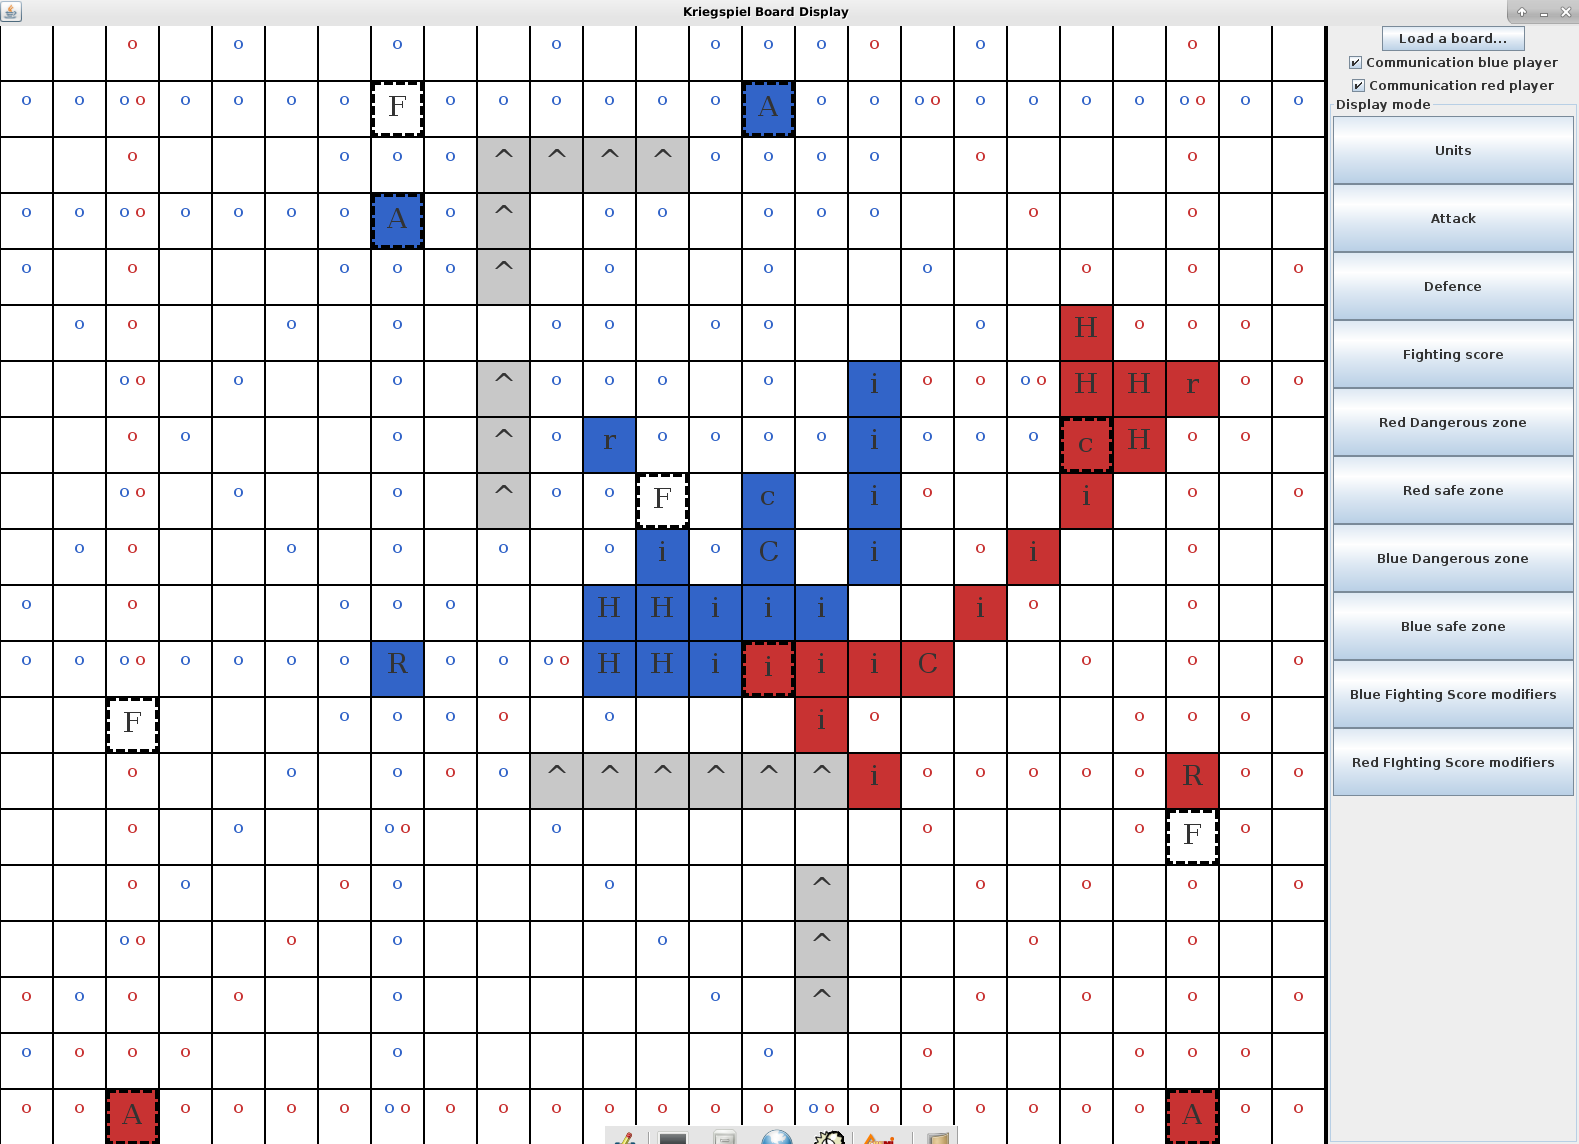
\includegraphics[width=0.5\textwidth]{pdp2014}
\end{figure}

\begin{figure}[h]
\caption{Potentiel d'attaque des unités rouges}
\centering
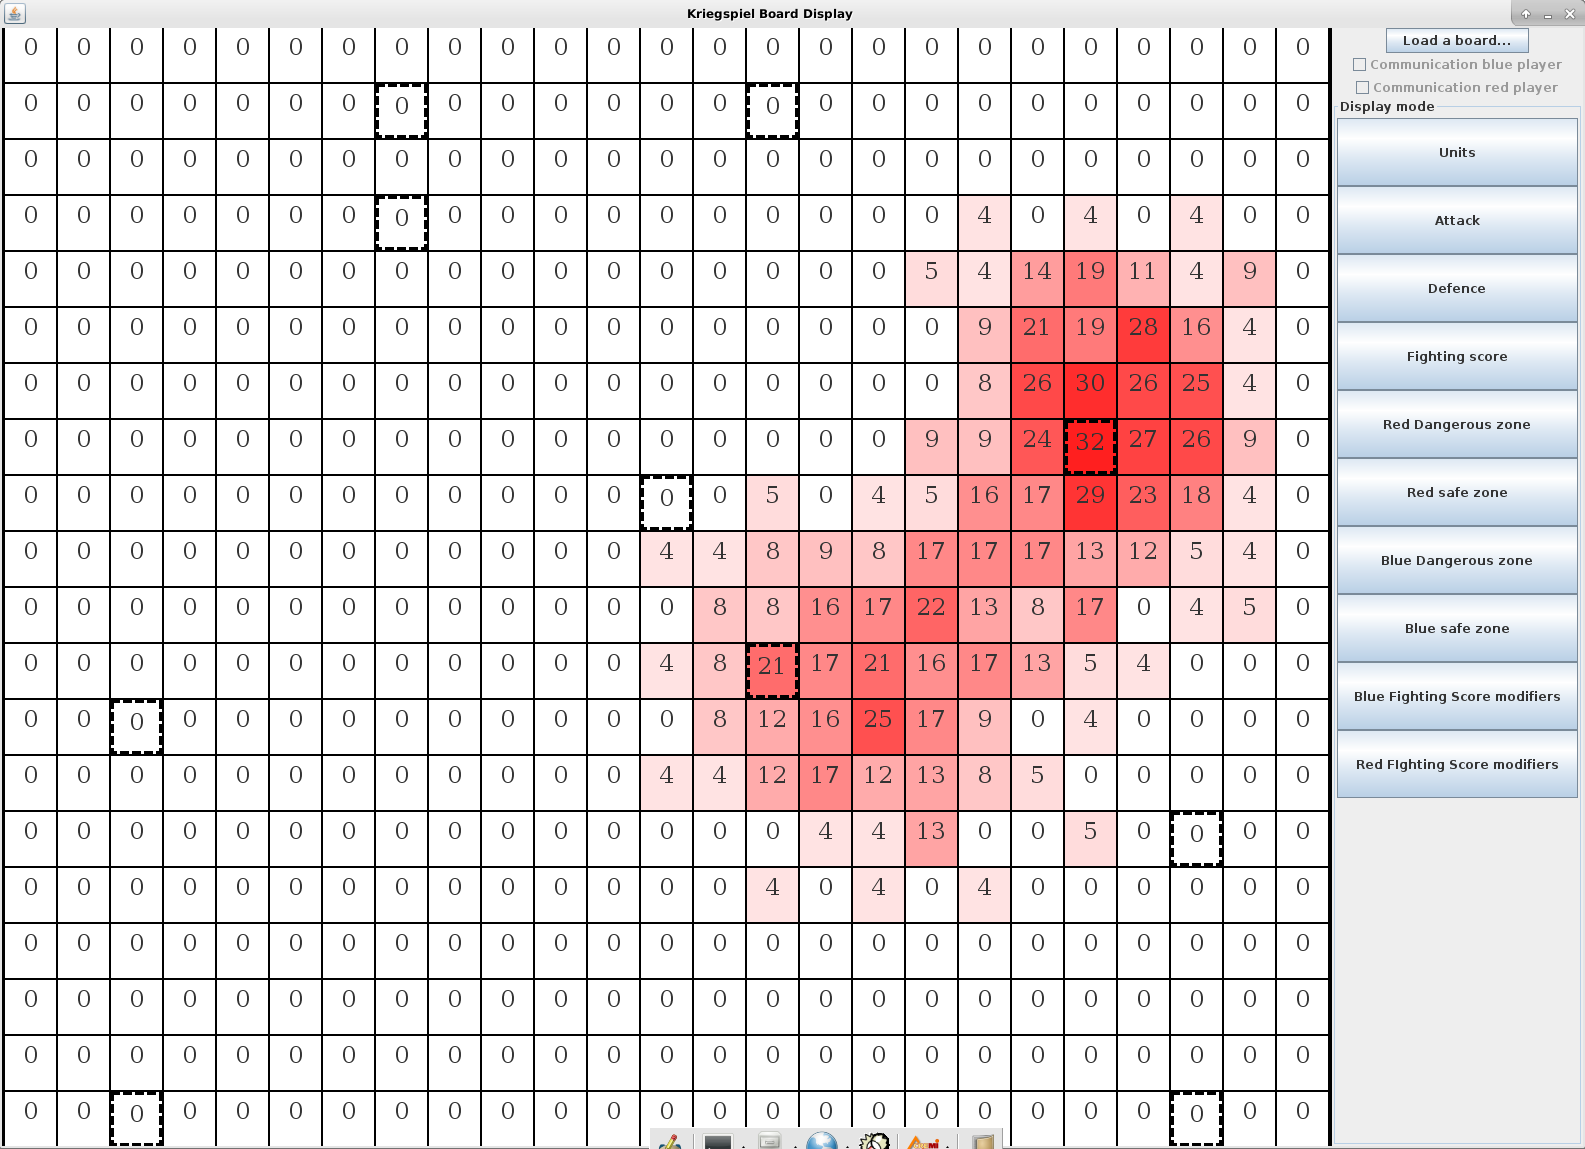
\includegraphics[width=0.5\textwidth]{pdp20142}
\end{figure}

\begin{figure}[!h]
\caption{Variation de potentiel de défense des unités bleues}
\centering
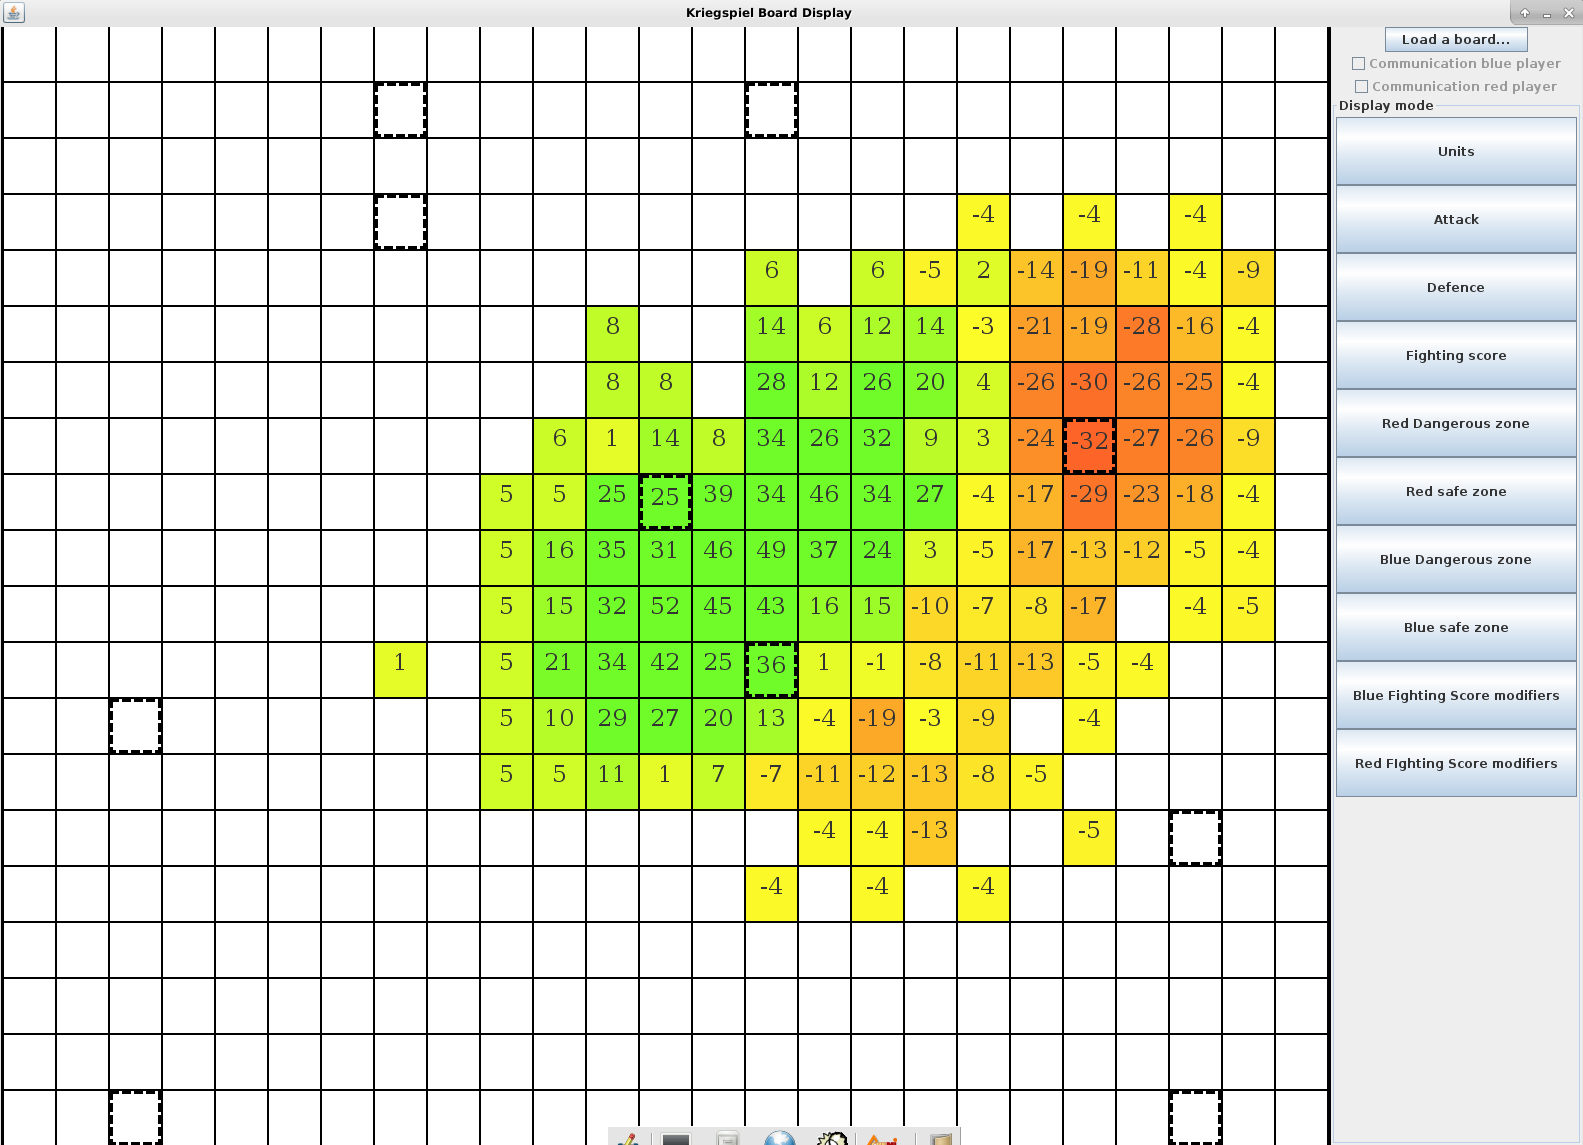
\includegraphics[width=0.5\textwidth]{pdp20143}
\end{figure}


\subsection*{Kriegspiel par RSG\cite{rsg}}
Ce projet n'est plus disponible sur le site de Radical Software Games, mais les sources restent cependant trouvables sur d'autres sites tiers. Il permettait de jouer en réseau contre un autre joueur au \textit{Jeu de la Guerre}, cependant des règles ont été simplifiées. Des aides visuelles sont présentes sur le plateau du jeu, permettant de voir les lignes de communication de chaque camp, ainsi que les cases où peut se déplacer une unité et si ces cases sont à portée d'une ligne de communication ou non. Il semble bien fonctionnel, mais il a été retiré du site pour une refonte, et semble malheureusement abandonné depuis.

\begin{figure}[!h]
\caption{Interface de Kriegspiel par RSG}
\centering
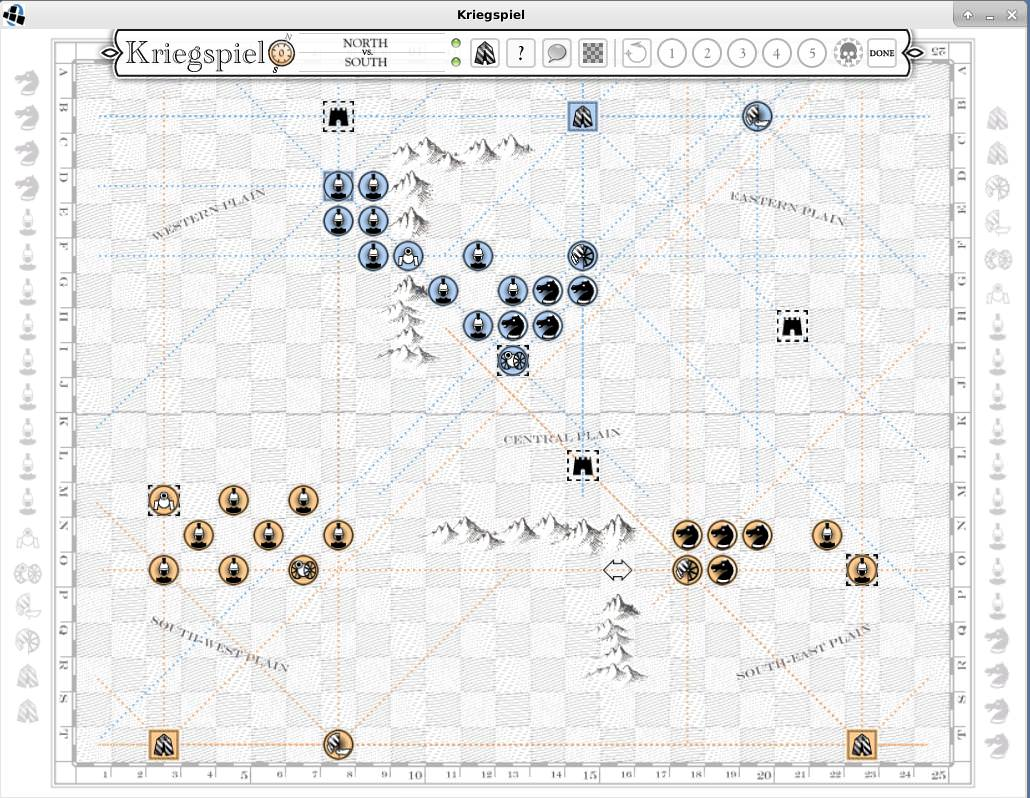
\includegraphics[width=0.9\textwidth]{rsg}
\end{figure}

\subsection*{Conclusion}
\`A notre connaissance, et après des recherches, nous pensons donc qu'il n'existe pas de version jouable du \textit{Jeu de la Guerre} actuellement disponible. Cependant il existe d'autres jeux semblables au jeu de Debord partageant le principe de simuler une guerre sur un plateau afin de revivre des batailles historiques et/ou de comprendre les tactiques derrière ces affrontements. On peut notamment citer \textit{DesertFox}\cite{desertfox} qui était à l'origine le jeu proposé pour ce sujet mais d'une complexité bien supérieure à celle du \textit{Jeu de la Guerre}. Nous devrons donc recréer tout du début, mais les projets que nous avons cités pourront tout de même nous servir dans notre réflexion sur comment mener à bien le notre, ainsi que quelques pistes notamment sur l'interface utilisateur.

% intro
% En plus du livre écrit par Debord, il existe déjà des documents liés à notre projet :

% \section{Kriegspiel}

% Le jeu \href{http://r-s-g.org/kriegspiel/index.php}{Kriegspiel} également basé sur le jeu de Guy Debord.

\chapter{Besoins fonctionnels}

\section{Définition des priorités}
\subsection{Besoins primaires} % Priorité 0

L'objectif premier consiste à mettre en place une version jouable, via la console, du \textit{Jeu de la Guerre} à l'aide d'un moteur de jeu implémentant les règles en restant le plus fidèle aux idées de Guy Debord. Ce moteur de jeu devra permettre d'affirmer si une action donnée par un joueur à un moment donné d'une partie est valide ou non. Cette implémentation devra pouvoir rendre possible l'extension du moteur pour les besoins secondaires et tertiaires.
\newline

%L'objectif premier à réaliser, et le grand pilier du projet, consiste à implémenter de façon informatique les règles du Jeu de la guerre en respectant autant que possible les idées de Guy Debord, dans une sorte de moteur de règles qui permet d'affirmer si un coup donné par un joueur à un moment donné d'une partie est valide ou non. Cette implémentation devra pouvoir rendre possible l'extension du moteur pour les besoins secondaires et tertiaires ainsi que posséder une interface permettant à un utilisateur d'interagir avec le programme.
%\newline

Les besoins et contraintes de programmation apportés par cette première partie sont les suivants :

\begin{enumerate}
\item Mettre en place un moteur de règle respectant les règles décrites dans le \textit{Jeu de la Guerre}.

\item Permettre à deux utilisateurs de jouer dans une même console à tour de rôle.

\item À son tour avant le début de la partie, l'utilisateur devra positionner ses unités sur le plateau sans que la position de l'armée adverse lui soit montrée.

\item Dans la phase de positionnement des unités, l'utilisateur pourra déplacer ses unités déjà placées sur le plateau sans limitation dans sa zone à l'aide de la commande permettant le déplacement d'une unité.

\item Les unités sont désignées de la façon suivante : (voir figure \ref{fig:commands})
	\begin{itemize}
	\item Le régiment d'infanterie : \texttt{I}
    \item Le régiment de cavalerie : \texttt{C}
    \item Le régiment d'artillerie à pied : \texttt{A}
    \item Le régiment d'artillerie à cheval : \texttt{Ac}
    \item L'unité de communication à pied : \texttt{R}
    \item L'unité de communication à cheval : \texttt{Rc}
    \item Une montagne : \texttt{M}
    \item Un col : \texttt{Co}
    \item Une forteresse : \texttt{F}
    \item Un arsenal : \texttt{Ar}
	\end{itemize}

\item À son tour, l'utilisateur devra proposer une action en utilisant la syntaxe suivante. Les actions disponibles dans un premier temps sont les suivantes (voir figure \ref{fig:commands}) :
	\begin{itemize}
    \item La position de chaque case est décrite par l'utilisateur à l'aide d'une ou plusieurs lettres suivi, sans espace, d'un nombre représentant respectivement l'axe des ordonnées et des abscisses. Ainsi, la case supérieure gauche est A1 et la case inférieure droite est T25.
    \item Positionner une unité au début de la partie : \texttt{set <U> <C1>} où \texttt{U} est le type de l'unité et \texttt{C1} la case où l'utilisateur veut la positionner.
	\item Déplacer une unité sur une case ciblée vers une autre case : \texttt{move <C1> <C2>} où \texttt{C1} est l'unité alliée ciblée, \texttt{C2} la case d'arrivée
    \item Attaquer une case en ciblant la case de l'unité attaquante : \texttt{attack <C1> <C2>} où \texttt{C1} est l'unité alliée ciblée, \texttt{C2} la case où se situe l'unité ennemie attaquée.
    \item Déclarer la fin de son tour : \texttt{end}
    \item Déclarer forfait : \texttt{surrender}
    \item Proposer un match nul : \texttt{pat}
    \item Accepter une requête : \texttt{Y}
    \item Refuser une requête : \texttt{N}
	\end{itemize}
    
\item Lorsqu'un déplacement est proposé, le programme devra lui même trouver un chemin valide pour y accéder.
\item Le programme générera et affichera un aperçu de la situation représentant l'état du plateau après chaque coup valide joué (nature de l'aperçu à définir ultérieurement, voir figure \ref{fig:prerelease}).

\item Afficher au début du prompt le numéro du joueur qui est en train de jouer.

\item Le programme ne sera pas sensible à la casse pour les entrées de l'utilisateur.


\end{enumerate}
% sémantique/commandes de l'utilisateur
% -Load
% -Save
% -Move
% -Attack
% (Spécifier des options de début de partie ?)
% (Placer les unités au début de la partie ?)
% 
%Si les besoins primaires consistent seulement dans l'implémentation d'un moteur de règle fonctionnel, il faut pouvoir lui donner un plateau, avec lequel il pourra communiquer, et donc prévoir aussi ça...

\subsection{Besoins secondaires} % Priorité 1
% revoir priorités again
Le projet se divise donc en deux parties, après avoir une version jouable du \textit{Jeu de la Guerre} entre deux utilisateurs sur une même console, il est désormais question d'ajouter des aides aux joueurs et des interactions avec l'interface graphique.

Il s'agit d'étendre l'implémentation actuelle pour permettre de pouvoir jouer une partie complète sur le programme en utilisant des aides à la compréhension d'une situation.

Ces aides permettront à l'utilisateur d'appréhender plus facilement et rapidement la situation de la partie, à savoir par exemple, mais peut-être pas limité à, le potentiel offensif et défensif de chaque case du plateau, la portée des lignes de communications, la portée d'attaque des unités. Ces aides ne devront pas être exclusivement visuelle et pourront être utilisées par un potentiel joueur artificiel plus tard.

L'utilisateur sera en mesure de jouer toute une partie via l'interface graphique à l'aide de sa souris. Il pourra ainsi interagir avec ses unités mais aussi sélectionner les aides à afficher/enlever sur le plateau à l'aide d'un menu déroulant par exemple.
\newline

Ainsi les besoins pour cette partie sont les suivants :

%Le joueur artificiel devra reconnaître l'ensemble des coups possibles à son tour, et pouvoir les jouer en pouvant utiliser des heuristiques qui seront détaillées dans les besoins tertiaires. Dans ce premier temps, on pourra par exemple, limiter ces heuristiques et plutôt jouer les coups de façon aléatoire.

\begin{enumerate}
\item Lorsqu'un coup est refusé par le moteur de règle, une explication du refus devra être affichée sur la console.

\item Sauvegarder l'état du plateau dans un fichier texte, en codage ASCII, en respectant un ordre logique des informations stockées, le fichier sera lisible par l'utilisateur. Cette action sera possible à l'aide de la commande : \texttt{save <File>}

\item Le fichier de sauvegarde aura le format suivant :
\begin{figure}[h]
\caption{Format de la sauvegarde}
\centering
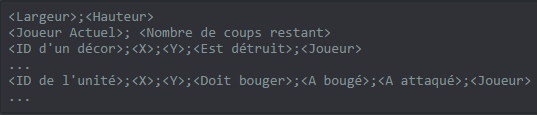
\includegraphics[width=0.8\textwidth]{saveFormat}
\end{figure}

%<Joueur Actuel> <Nombre de coups restant>
%<ID d'un décor>;<X>;<Y>;<Est cassé>;<Joueur>
%.
%<ID de l'unité>;<X>;<Y>;<Doit bouger>;<A bougé>;<A attaqué>;<Joueur>
%.

\item Instancier une partie à partir d'un fichier texte, en codage ASCII, respectant l'ordre logique des informations décrit par la sauvegarde. Cette action sera possible à l'aide de la commande : \texttt{load <File>}

\item Annuler la dernière action effectuée par l'utilisateur à l'aide de la commande : \texttt{revert}

\item Permettre le déplacement d'une unité qui initiera une attaque à l'issue de ce mouvement à l'aide la commande : \texttt{charge <C1> <C2> <C3>} où \texttt{C1} est l'unité alliée ciblée, \texttt{C2} la case d'arrivée de l'unité et \texttt{C3} la case où se situe l'unité ennemie attaquée.

\item Afficher/enlever les lignes de communications sur l'aperçu du plateau à l'aide de la commande : \texttt{toggleCom}

\item Afficher/enlever le potentiel d'attaque de l'utilisateur sur chaque case si il est différent de 0 à l'aide de la commande : \texttt{toggleAtk}

\item Afficher/enlever le potentiel de défense de l'utilisateur sur chaque case si il est différent de 0 à l'aide de la commande : \texttt{toggleDef}

\item Sélectionner une unité à l'aide d'un clic gauche de la souris, la case ainsi sélectionnée sera mis en évidence (surbrillance, bords plus gros, ...).

\item Sélectionner une case vide à l'aide d'un clic gauche de la souris lorsqu'une unité est sélectionnée déclenche son déplacement si celui-ci est possible.

\item Sélectionner une unité adverse lorsqu'une unité est sélectionnée déclenche une attaque si elle est possible sur la case ciblée.

%\item Sélectionner une case vide à l'aide d'un clic gauche de la souris permet de déselectionner une case précédemment sélectionnée.

\item Des boutons sur le côté du plateau ou un menu déroulant seront disponibles permettant d'afficher ou d'enlever certains modes rajoutant de l'information visuelle sur le plateau. Ces modes seront en partie constitués des précédents besoins décrits à savoir l'affichage du potentiel d'attaque et/ou de défense sur chaque case du plateau si cette valeur est différente de 0.

\item Des menus déroulant permettront d'accéder aux fonctionnalités de sauvegarde et de chargement d'un fichier comme décrit dans les besoins primaires.

\item Lors de la phase de positionnement des unités, l'utilisateur pourra choisir une unité parmi celles se trouvant dans un cadre sur l'un des côtés du plateau, pour la positionner sur la case du plateau choisie à l'aide d'un clic gauche de la souris.

\item Toujours durant cette phase, l'utilisateur pourra repositionner une unité sur le plateau sur une autre case, un échange de position se fera si la case ciblée est occupée par une unité alliée.

%%% Priorité 1 - Interface minimale (console) pour joueurs
% Afficher et expliquer les règles vérifiées et leur validité
% + étape de validation par le joueur d'un coup affirmé valide ? (test/simulation de coup)

  %\item Permettre à deux utilisateurs de jouer dans une même console à tour de rôle.
  
  %\item À son tour, l'utilisateur devra proposer une action en utilisant une syntaxe à définir.
  
  %\item Le programme générera et affichera un aperçu de la situation représentant l'état du plateau après chaque coup valide joué (nature de l'aperçu à définir ultérieurement).
  
  %\item Toujours avec cette syntaxe, un joueur devra pouvoir annuler les derniers coups qu'il a joué, jusqu'à revenir au début de son tour s'il le souhaite. (Ce mécanisme pourra être implémenté à l'aide d'une pile des instances du plateau pendant ce tour). % voir avec test/simulation
  
  %\item Un joueur pourra sauvegarder l'état du plateau dans un fichier en respectant un ordre logique des informations stockées, lisible par l'utilisateur.
  %\item Un joueur pourra générer une instance du jeu à partir d'un fichier suivant un format défini.
  %\item Une première IA sera implémentée. Elle sera en lien avec le moteur de règle et pourra récupérer la liste des coups valides, pourra proposer des actions au jeu et devra pouvoir être étendable. %(étendue facilement)

\end{enumerate}

% Priorité 2 - "bonus" visuels (axes de communication, pértinence de cases et coups, etc)

\subsection{Besoins tertiaires} % Priorité 2
%Cette dernière partie du projet se focalise sur le joueur artificiel exclusivement, afin de pouvoir le faire jouer de façon efficace en utilisant des notions tactiques et stratégiques \cite{AI2009}. Il faudra probablement faire interpréter une situation donnée au joueur artificiel pour que celui-ci prenne une décision pertinente dans un temps réduis. On pourra penser par exemple à représenter les unités des deux joueurs par des "ensembles d'unités à un certain potentiel".
Dans cette partie, il s'agira de se focaliser sur un analyseur, utilisant des données telle que la cartographie des coefficients d'attaque, dont le but sera de pouvoir calculer un ou plusieurs coups à partir d'une situation donnée, en utilisant des notions stratégiques \cite{AI2009} pour lui faire mettre en place une tactique.
\newline 

M. Narbel nous a notamment indiqué les deux besoins concernant une stratégie potentielle pour un joueur artificiel : %TBC
\newline

\begin{itemize}

% Ajouter des ouvrages de référence
\item Évaluation ("compréhension") d'une position (statique),
   (Spatial Reasoning\cite{spatial-reasoning} - Potential fields - PathFinding)
   Détermination de "points décisifs".  Représentation graphique de
   cette évaluation (attaque, défense, communications).

\item Évaluation ("compréhension") d'une suite de mouvements (dynamique).
   Prise en compte de techniques de planification (Planning).
   Représentation graphique de cette évaluation.

\end{itemize}

Pour le rendu final, au moins une stratégie et une tactique seront attendues, pouvant être utilisées en même temps, à savoir :
\begin{itemize}
\item Une stratégie permettant de trouver le chemin le plus efficace pour atteindre les arsenaux de l'adversaire (analyse des "vallées" ou faiblesses dans la formation adverse pour atteindre l'objectif).
\item Une tactique permettant d'obtenir une configuration optimale dans la planification d'une attaque ou d'une défense (utilisation d'une cartographie des potentiels d'attaque et de défense).
\end{itemize}

D'autres stratégies pourront être mises en place si le temps le permet, à savoir mesurer l'agressivité et le positionnement des troupes de l'adversaire (réduction à une dimension pour chacun des axes), et de détecter les tactiques "commando", comme remarqué avec le détachement de l'unité de Cavalerie dans la partie présentée par Debord dans son livre (voir \cite{jdg}, pages 11-127).

Ces stratégies et tactiques pourront être utilisées comme représentation graphique pour conseiller le joueur (aperçus types "schémas militaires"), ainsi que comme une série d'indications pour un potentiel joueur artificiel.
   
% Une première IA sera implémentée. Elle sera en lien avec le moteur de règle et pourra récupérer la liste des coups valides, pourra proposer des actions au jeu et devra pouvoir être étendable. %(étendue facilement)

% TODO : Développer

\begin{figure}[h]
\caption{\'Ebauche d'interface commande et d'aperçu de l'état du plateau}
%\caption{\'Ebauche d'interface commande et d'aperçu de situation pour la première \textit{release}}
\centering
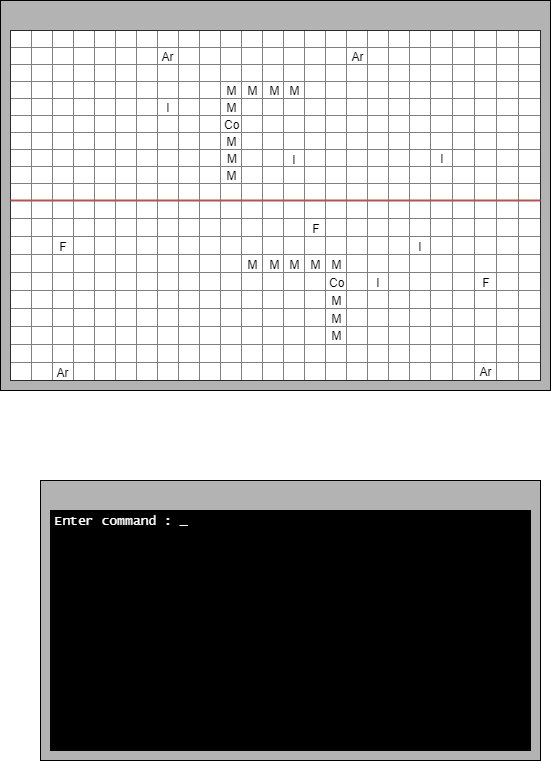
\includegraphics[width=0.5\textwidth]{interface_pdp2}
\label{fig:prerelease}
\end{figure}

\begin{figure}[h]
\caption{Commandes et identifiants des unités et terrains employés}
\centering
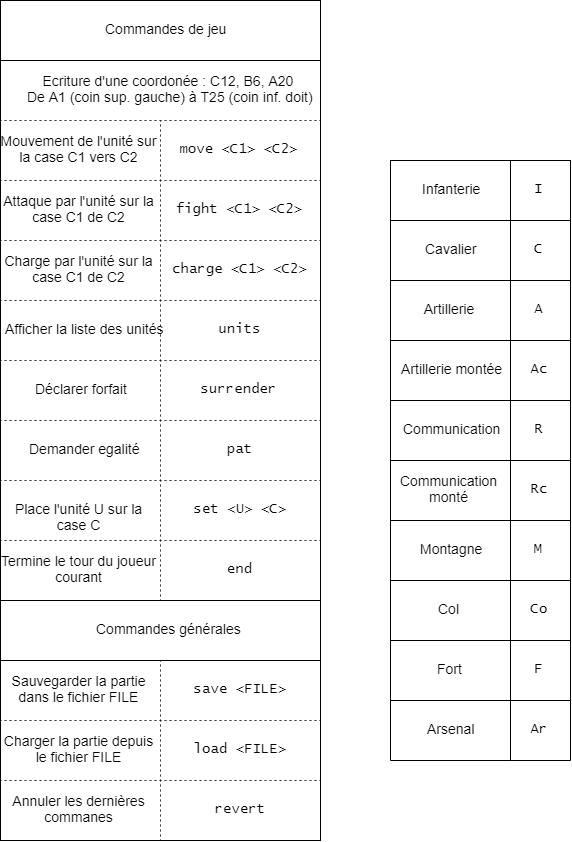
\includegraphics[width=0.5\textwidth]{interface_pdp}
\label{fig:commands}
\end{figure}

\begin{figure}[h]
\caption{\'Ebauche d'interface utilisateur graphique pour la \textit{release} finale}
\centering
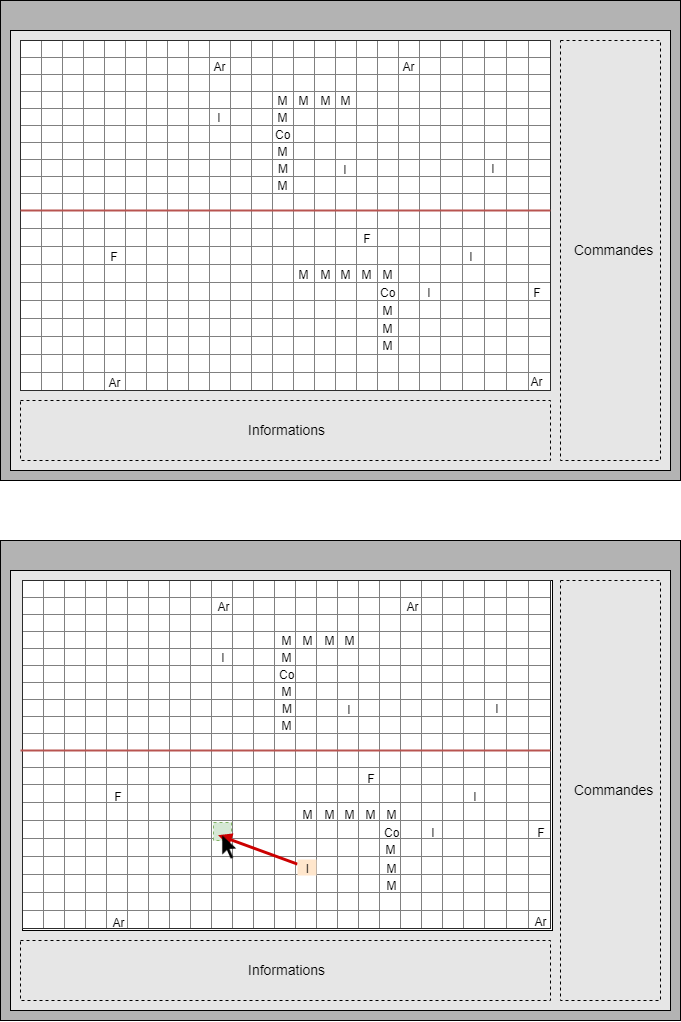
\includegraphics[width=0.8\textwidth]{interface_pdp3}
\label{fig:release}
\end{figure}

\begin{figure}[h]
\caption{Scénario d'utilisation pour un coup proposé}
\centering
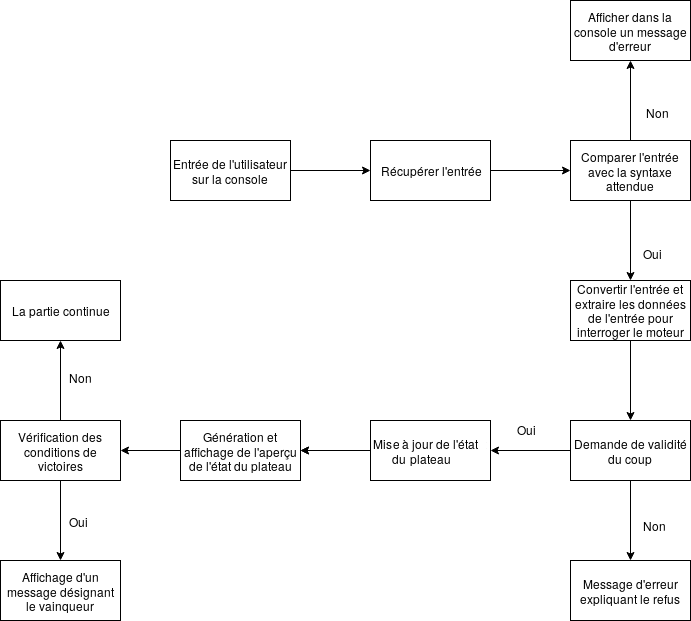
\includegraphics[width=0.8\textwidth]{scenario}
\label{fig:scenario1}
\end{figure}

%\begin{figure}[h]
%\caption{Diagramme de séquence pour un coup valide proposé}
%\centering
%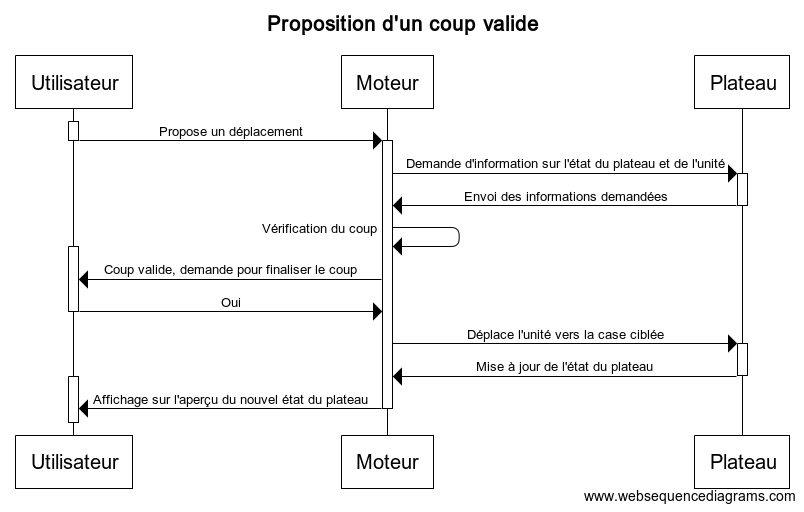
\includegraphics[width=0.8\textwidth]{sequence}
%\label{fig:scenario1}
%\end{figure}


% \section{Besoins accessoires}
% % wtf
% Pour améliorer le projet si les besoins les plus importants ont été accomplis, plusieurs idées peuvent être mises en oeuvre :

% \begin{itemize}
% \item Une représentation graphique 2D du jeu, avec diverses aides visuelles telles que l'affichage des lignes de communication et la puissance des unités.
% \end{itemize}


% Classer les règles du jeu et l'ordre dans lequel on doit les implémenter

\chapter{Besoins non-fonctionnels}

\begin{enumerate}
% \item Il devra être fait mention de Guy Debord en tant qu'auteur du Jeu de la Guerre
\item Le code du moteur de règles devra avoir un certain degré de généricité et de modularité pour pouvoir altérer les règles du jeu lors du développement ou même après la release finale (voir figure \ref{fig:modules} pour une idée de la modularité attendue).

\item Le temps d'attente entre un coup proposé et sa validité évaluée par le moteur de règle devra être de l'ordre de la seconde.

% \item Le temps d'attente entre le début et la fin du tour de l'IA ne devra pas excéder 10 secondes.

\item Le jeu doit fonctionner sur un système UNIX.

\item Le jeu sera codé dans le langage de programmation Java, et Scala pour les interfaces graphiques.


\begin{figure}[h]
\label{fig:modules}
\caption{Présentation des modules du programme.}
\centering
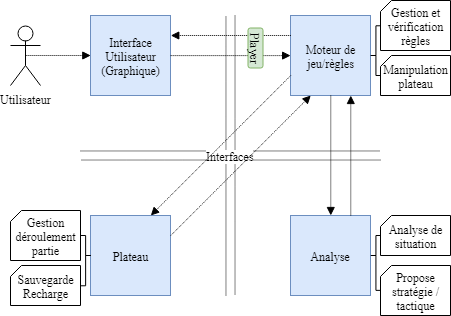
\includegraphics[width=0.8\textwidth]{pdp_modules}
\end{figure}

\item Le module de moteur de règles sera composé d'un ensemble de règles et s'occupe de modifier l'état du plateau sur le déroulement d'une partie.

\item Le module d'interface utilisateur offrira un environnement utilisable par l'utilisateur pour interagir avec le jeu. Les interactions avec le moteur de jeu seront définies par une interface (représentée par \texttt{Player}) qui sera aussi utilisée aussi bien que par un joueur humain que par un potentiel joueur artificiel. Cet environnement sera dans un premier temps une interface console affichant l'état du plateau dans une fenêtre à part, puis une interface graphique après la première release. %%TODO ?

% \item Le module d'IA sera composé de "comportements" et interagira avec le moteur de règles pour avoir les informations sur l'état de la partie pour décider du coup à jouer. Les fonctionnalités pour obtenir ces informations pourront être utilisées aussi par le module d'interface utilisateur afin d'afficher les aides visuelles comme les portées d'attaque, les valeurs de défense des unités, etc...

\item Le module d'Analyse permettra d'obtenir des informations et données stratégiques et tactiques sur une situation donnée et sur les tours précédents. L'idéal serait de pouvoir proposer des stratégies ou tactiques à partir de ces informations, pouvant être ultimement employé par un joueur artificiel.

\item Le module de plateau est une sorte de conteneur qui s'occupe de gérer l'état du plateau, de l'exporter et de l'importer. Il ne doit pas être accessible par les autres classes Analyse et Interface Utilisateur pour éviter la perte de cohérence sur le déroulement de la partie. Restreindre l'accès au Plateau uniquement au moteur de jeu force les autres modules à passer par la vérification des règles avant d'agir sur le terrain.

\item Une couverture des tests sur les différents modules du jeu est attendue lors du développement. Ces tests devront être implémentés par les développeurs travaillant sur leur module au fur et à mesure.
%(instances)

\item Des tests en boîte noire devront être fournis, permettant de valider les interactions entre l'utilisateur et le programme. Certains de ces tests se baseront sur les configurations du plateau de la partie décrite dans le livre de Debord (voir \cite{jdg}, pages 14-24), notamment pour vérifier si l'état du plateau résultant du test sur l'état initial est bien conforme à ce qui est décrit. Cette partie servira aussi de témoin principal pour confirmer la validité des règles implémentées.

\item Le développement des différentes étapes non triviales devra être conduit par groupes de 2 (voir le diagramme \ref{fig:gantt}) développeurs pour garder une cohérence, pas plus pour éviter les ralentissements sur une seule partie du code, mais pas moins non plus pour avoir un code maintenable et compris par plusieurs développeurs.

\item Les deux dernières semaines du projet seront réservées à la rédaction du mémoire ainsi que pour compenser le retard éventuel généré lors du développement.
\end{enumerate}

\begin{figure}[h]
\caption{Diagramme de Gantt - Représentant les effectifs par tâche}
\centering
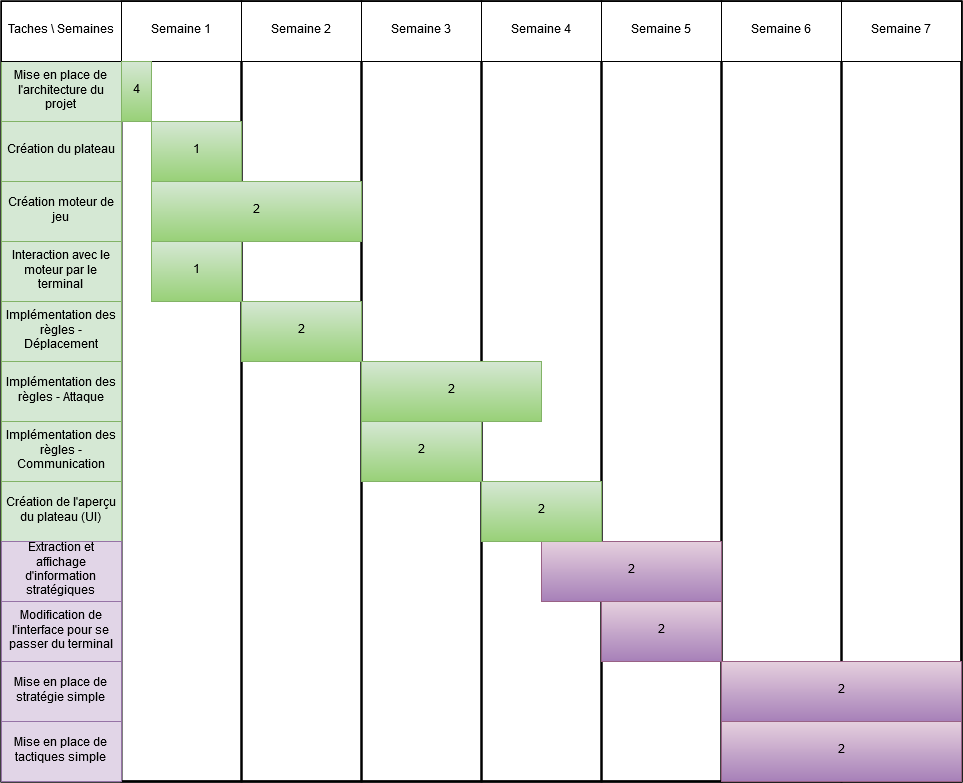
\includegraphics[width=0.8\textwidth]{Gantt}
\label{fig:gantt}
\end{figure}

\bibliographystyle{plain}
\bibliography{bib}


%\chapter{}

%You can upload a \verb|.bib| file containing your BibTeX entries, created with JabRef; or import your \href{https://www.overleaf.com/blog/184}{Mendeley}, CiteULike or Zotero library as a \verb|.bib| file. You can then cite entries from it, like this: \cite{greenwade93}. Just remember to specify a bibliography style, as well as the filename of the \verb|.bib|.

%You can find a \href{https://www.overleaf.com/help/97-how-to-include-a-bibliography-using-bibtex}{video tutorial here} to learn more about BibTeX.

%%tableau
%%\begin{table}
%\centering
%\begin{tabular}{l|r}
%Item & Quantity \\\hline
%Widgets & 42 \\
%Gadgets & 13
%\end{tabular}
%\caption{\label{tab:widgets}An example table.}
%\end{table}

%%img
%%
%\begin{figure}
%\centering
%\includegraphics[width=0.3\textwidth]{frog.jpg}
%\caption{\label{fig:frog}This frog was uploaded via the project menu.}
%\end{figure}
%%
\end{document}